\documentclass[a4paper,11pt]{article}
\usepackage{amsmath,amsthm,amsfonts,amssymb,amscd,amstext,vmargin,graphics,graphicx,tabularx,multicol} \usepackage[french]{babel}
\usepackage[utf8]{inputenc}  
\usepackage[T1]{fontenc} 
\usepackage[T1]{fontenc}
\usepackage{amsmath,amssymb}
\usepackage{pstricks-add,tikz,tkz-tab,variations}
\usepackage[autolanguage,np]{numprint} 
\usepackage{color}
\usepackage{ulem}

\setmarginsrb{1.5cm}{0.5cm}{1cm}{0.5cm}{0cm}{0cm}{0cm}{0cm} %Gauche, haut, droite, haut
\newcounter{numexo}
\newcommand{\exo}[1]{\stepcounter{numexo}\noindent{\bf Exercice~\thenumexo} : \marginpar{\hfill /#1}}
\reversemarginpar


\newcounter{enumtabi}
\newcounter{enumtaba}
\newcommand{\q}{\stepcounter{enumtabi} \theenumtabi.  }
\newcommand{\qa}{\stepcounter{enumtaba} (\alph{enumtaba}) }
\newcommand{\initq}{\setcounter{enumtabi}{0}}
\newcommand{\initqa}{\setcounter{enumtaba}{0}}

\newcommand{\be}{\begin{enumerate}}
\newcommand{\ee}{\end{enumerate}}
\newcommand{\bi}{\begin{itemize}}
\newcommand{\ei}{\end{itemize}}
\newcommand{\bp}{\begin{pspicture*}}
\newcommand{\ep}{\end{pspicture*}}
\newcommand{\bt}{\begin{tabular}}
\newcommand{\et}{\end{tabular}}
\renewcommand{\tabularxcolumn}[1]{>{\centering}m{#1}} %(colonne m{} centrée, au lieu de p par défault) 
\newcommand{\tnl}{\tabularnewline}

\newcommand{\trait}{\noindent \rule{\linewidth}{0.2mm}}
\newcommand{\hs}[1]{\hspace{#1}}
\newcommand{\vs}[1]{\vspace{#1}}

\newcommand{\N}{\mathbb{N}}
\newcommand{\Z}{\mathbb{Z}}
\newcommand{\R}{\mathbb{R}}
\newcommand{\C}{\mathbb{C}}
\newcommand{\Dcal}{\mathcal{D}}
\newcommand{\Ccal}{\mathcal{C}}
\newcommand{\mc}{\mathcal}

\newcommand{\vect}[1]{\overrightarrow{#1}}
\newcommand{\ds}{\displaystyle}
\newcommand{\eq}{\quad \Leftrightarrow \quad}
\newcommand{\vecti}{\vec{\imath}}
\newcommand{\vectj}{\vec{\jmath}}
\newcommand{\Oij}{(O;\vec{\imath}, \vec{\jmath})}
\newcommand{\OIJ}{(O;I,J)}

\newcommand{\bmul}[1]{\begin{multicols}{#1}}
\newcommand{\emul}{\end{multicols}}


\newcommand{\reponse}[1][1]{%
\multido{}{#1}{\makebox[\linewidth]{\rule[0pt]{0pt}{20pt}\dotfill}
}}

\newcommand{\titre}[5] 
% #1: titre #2: haut gauche #3: bas gauche #4: haut droite #5: bas droite
{
\noindent #2 \hfill #4 \\
#3 \hfill #5

\vspace{-1.6cm}

\begin{center}\rule{6cm}{0.5mm}\end{center}
\vspace{0.2cm}
\begin{center}{\large{\textbf{#1}}}\end{center}
\begin{center}\rule{6cm}{0.5mm}\end{center}
}



\begin{document}
\pagestyle{empty}
\titre{Contrôle 3 : Transformations et homothétie}{Nom}{Prénom}{Date}{Classe}

\vspace*{1cm}

\exo{4}
Chacun des triangles 2, 3, 4 et 5 est obtenu à partir du triangle 1 à l'aide d'une symétrie axiale, d'une symétrie centrale, d'une translation ou d'une rotation.\\

\textbf{Recopier}  les  quatre  phrases  suivantes  et \textbf{compléter} :
\bmul{2}

\noindent \q  L'image  du  triangle  1  par  la  symétrie axiale d'axe ... est le triangle ...\\
\q  L'image  du  triangle  1  par  la  symétrie centrale de centre ... est le triangle ...\\
\q L'image du triangle 1 par la translation de vecteur ... est le triangle ...\\
\q Le triangle 1 a pour image le triangle 4 par la rotation de centre ... et d'angle ... (le sens   de   la   rotation   est   indiqué   par   la flèche).\\



\columnbreak


\includegraphics[scale=0.7]{exotranf1.eps} 

\emul

\vspace*{1cm}


\exo{2}
Ci-dessous, sont représentées 6 tasses de cafés obtenues par homothétie de la tasse $C_{0}$ :\\

\begin{center}
 \includegraphics[scale=0.75]{tasse.eps}
 \end{center} 

\noindent \initq \q Noter sur la figure $C_{1}$ la tasse obtenu par homothétie de la tasse $C_{0}$ de centre O et de rapport 2.\\
\q Noter sur la figure $C_{3}$ la tasse obtenu par homothétie de la tasse $C_{0}$ de centre O et de rapport 0,6.\\
\q Noter sur la figure $C_{4}$ la tasse obtenu par homothétie de la tasse $C_{0}$ de centre P et de rapport 0,4.\\
\q Noter sur la figure $C_{5}$ la tasse obtenu par homothétie de la tasse $C_{0}$ de centre P et de rapport 2.\\

\newpage


\exo{4}
\initq \q Construire  l'image du triangle gris par l'homothétie de centre O et de rapport k = 2.\\
\q Construire  l'image du triangle gris par l'homothétie de centre O et de rapport $k=\dfrac{1}{2}$.

\begin{center}
\includegraphics[scale=1]{homothetie.eps} 
\end{center}



\exo{4} Tracer $F_{2}$ l'image de la figure $F_{1}$ par l'homothétie de centre F et de rapport k = -1,5.\\
Tracer $F_{3}$ l'image de la figure $F_{1}$ par l'homothétie de centre F et de rapport k = -0,75.

\begin{flushright}
\includegraphics[scale=0.75]{homothetie2.eps} 
\end{flushright}


\newpage

\vspace*{1cm}


\exo{2,5}
Soit MONA un rectangle de longueur 12 m et de largeur 5 m et M'O'N'A' son image par une homothétie de rapport k = 6.\\

\noindent \initq \q Calculer l'aire du rectangle MONA.\\
\q Sans tracer de figures et en utilisant une propriété du cours, calculer l'aire du rectangle M'O'N'A'. Quel est le facteur d'agrandissement d'aire ? \textbf{(Justifier votre calcul)}\\

\vspace*{1cm}
\exo{4.5}

Les droites (AE) et (OC) sont sécantes en B. \\
Le triangle ABC est l'image du triangle OBE par une homothétie.

\begin{center}
\includegraphics[scale=1]{homorapport.eps}
\end{center} 



\initq 
\noindent \q Quel est le centre de cette homothétie?\\
\q Quel est le rapport de cette homothétie? Justifier votre réponse.\\
\q Calculer la longueur du segment [BE] et du segment [OE]. Justifier votre réponse.\\
\q Que peut-on dire des droites (AC) et (OE) ? Justifier votre réponse.\\



\end{document}
